% !TEX root = ../../main.tex

\section{Compliance in porous crystals}

\subsection{Examining the assumption of an inert adsorbent}

Adsorption induced changes in porous media have been known
to occur for over 90 years~\cite{mcbainNatureInfluenceHumidity1927},
with both clays, coals and polymers undergoing swelling during gas
or vapour uptake~\cite{gorAdsorptioninducedDeformationNanoporous2017}.
However, the effect upon the macroscopic properties of the material is 
often negligibly small and of little consequence to industrial adsorption
processes. Studies of this aspect of porous adsorbents have therefore
been scarce in the large part of the 20\textsuperscript{th} century,
likewise influenced by lack of sufficiently accurate methods for 
characterising and modelling such occurrences.

In recent years, the advent of reference materials, 
highly sensitive methods such as synchrotron-grade X-rays and computer-aided
computational techniques such as DFT has put at our disposal the tools 
required to study these transformations. 
Together with the discovery of their role in natural and industrial 
processes e.g.\ the swelling of shale during natural gas extraction,
maturation of concrete and perspectives afforded by novel porous materials,
these factors have generated renewed scientific interest in material
compliance.

The driving process behind the phenomenon is stress-induced framework 
strain. In-depth studies~\cite{beringAlterationZeoliteGranule1977} 
have revealed that most porous materials posses some small
degree of compliance, with \textit{in-situ} dilatometry going so far as to 
obtain pore size distributions from accurate volume
changes~\cite{reichenauerExtractingPoreSize2001}. Most flexible 
processes can be likened to continuous order processes. It is, however,
with the discovery of large scale flexibility in MOFs such as 
MIL-53 and linker-controlled gate opening like in ZIF-8, 
where the transformation between the different framework 
states occurs suddenly at precise points in the loading curve,
which has shown that compliance may also take the form of 
a first-order transition. Such types of transformations are
desirable~\cite{kitagawaFunctionalPorousCoordination2004} due to 
their highly specific response. The possible dependence 
of flexibility on other stimuli, such as light, mechanical pressure,
temperature, magnetic fields may allow for precise tuning of 
structural changes. As such, it is reasonable to state that
the mobility of the solid phase can no longer be ignored.

\subsection{Flexibility in metal organic frameworks}

Since the highlight of compliance in porous coordination polymers 
in the report of~\citet{kitauraPorousCoordinationPolymerCrystals2003},
much progress has been made in the synthesis and understanding
of this phenomena. An exhaustive review of MOF flexibility is 
outside the scope of this thesis, with the field progressing 
rapidly enough to generate a wealth of critical
literature~\cite{schneemannFlexibleMetalOrganic2014, %
fereyHybridPorousSolids2008, liMetalOrganicFrameworks2012, %
haldarInterpenetrationCoordinationPolymers2015, %
stassenUpdatedRoadmapIntegration2017, %
vanduyfhuysThermodynamicInsightStimuliresponsive2018}.
Some of the known types of structural flexibility encountered in MOFs
will be briefly discussed, with a summary evident in \autoref{dut:fgr:flex-types}. 

\begin{figure}[htb]
    \centering
    
    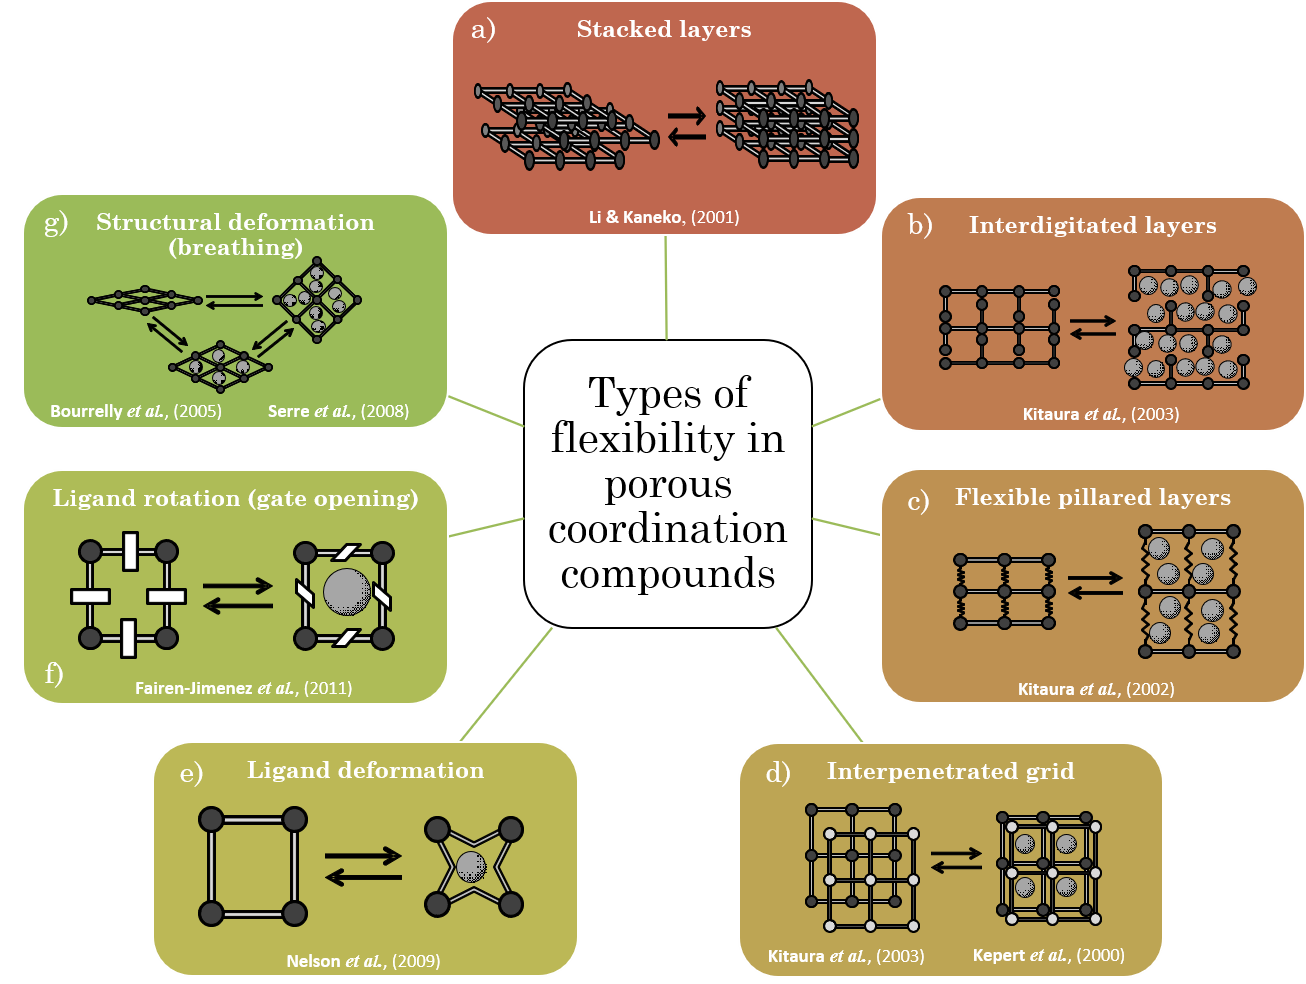
\includegraphics[width=\textwidth]{flexibility-types}%
    \caption{A visual summary of the types of flexibility
    which are documented in MOFs, as detailed in 
    (a)~\citet{liHydrogenBondregulatedMicroporous2001}
    (b)~\citet{kitauraPorousCoordinationPolymerCrystals2003}
    (c)~\citet{kitauraPillaredLayerCoordinationPolymer2002}
    (d)~\citet{kepertVersatileFamilyInterconvertible2000,%
    kitauraPorousCoordinationPolymerCrystals2003}
    (e)~\citet{nelsonSupercriticalProcessingRoute2009}
    (f)~\citet{fairen-jimenezOpeningGateFramework2011}
    (g)~\citet{bourrellyDifferentAdsorptionBehaviors2005, %
    serreExplanationVeryLarge2007}}%
    \label{dut:fgr:flex-types}
    
\end{figure}

Layer separation, as is the case in interdigitated 

Finally, MOFs can lead to structural flexibility which does not
require any volume changes in the unit cell. The rotation of linkers
can act as gating for different guests, allowing entry of probes
larger than the window size would suggest or preferential adsorption
of a gas which has the right property to act as a ``key'' from 
a mixture~\cite{seoPillaredLayerCoordinationPolymer2009}. 
The former effect might lend itself to temperature 
controlled storage and release of gasses~\cite{bunzenAchievingLargeVolumetric2018}
and is common in zeolitic imidazole frameworks 
(ZIFs)~\cite{fairen-jimenezOpeningGateFramework2011}.


, as they have been shown to undergo massive and 
reversible structural deflections, while retaining their 
crystalinity

The discovery of the so-called ``breathing'' type of structural
deformation in the MIL-53 family of materials has shown that 

\subsection{Describing adsorbate compliance}

The induced mechanistic phenomena are a result of several competing
effects, a sub-monolayer contraction~\cite{daceyVolumeChangesSaran1971} resulting
from micropore bridging or surface stresses, followed by a monotonic 
expansion with the gradual decrease of the solid-fluid interface energy
also known as the Bangham effect~\cite{banghamExpansionCharcoalAccompanying1928}. 
Such behaviour is highly dependent of pore size, geometry and anisotropy,
with condensation in macropores a further complex source of 
strain~\cite{dolinoAdsorptionStrainsPorous1996, ambergSTUDYADSORPTIONHYSTERESIS1952, %
guntherNovelInsightsNanopore2008}. The degree of adsorption induced
changes in a structure is generally a function of its porosity, with very high 
surface area materials such as aerogels capable of undergoing up 
to 30\% deformation~\cite{reichenauerNitrogenSorptionAerogels2001}.

The type of
swelling, contraction and expansion usually follows a second order
transition.

Finding a suitable model that would predict such structural changes
has remained a challenge. A successful model for 
~\cite{neimarkStressBasedModelBreathing2010}
~\cite{gorAdsorptionInducedDeformationMesoporous2010}
Nevertheless a complete theory of adsorption-deformation 
which can fully predict the changes in the measured enthalpy of 
adsorption and the mechanistic behaviour of theoretical structures
has remained elusive.


However, the most promising perspective for such materials come from


\subsection{Consequences and applications of compliance}

The usefulness of such phenomena have been long recognised as potential
sensors or actuators, initially by nature itself, with humidity induced 
swelling acting to open pine cones~\cite{dawsonHowPineCones1997}. 
More recently similar sensing devices based on adsorption induced 
strain in mesoporous silica have been 
developed~\cite{boudotConvertingWaterAdsorption2016, %
ganserCantileverBendingBased2016} which show promise for use 
in micromechanical systems. From a gas storage and separation 
point of view, changes in the adsorbent structure may be crucial 
for process improvement. Pressure swing adsorption (PSA) is heavily 
dependent on the working capacity of the adsorbent used, or the
difference between loading at the operation pressure and at the 
regeneration pressure. In this case, an S-shaped isotherm, with 
the vertical part of the slope in the aforementioned pressure 
range would lead to high process efficiency gains by eliminating material
``dead volume adsorbed''~\cite{schneemannFlexibleMetalOrganic2014}. 
In a temperature swing process (TSA), where 
the regeneration is performed through heating of the adsorbent 
bed, the key parameter is the integral enthalpy of adsorption, a measure 
of the energy requirements for the process. As a part of the chemical 
potential of the adsorbed phase is used by the mechanical contraction
of the material, flexible adsorbents have the potential of
intrinsic thermal management, reducing the energy cost~\cite{masonMethaneStorageFlexible2015}.
Both effects are equally applicable to the storage of pure 
gasses, increasing the storage capacity and work required to
desorb the gas.
Finally, swelling of clays upon gas adsorption 
is quickly becoming a research interest as extraction of shale 
deposits is becoming common. In particular, the attractive option
of combined carbon capture and methane recovery implemented 
through pumping of carbon dioxide into reservoirs leads to swelling-induced
loss of porosity and well blocking due to the increased strain 
by \ce{CO2} in comparison to methane. 
